\documentclass[titlepage, a4paper]{article}
\usepackage[english]{babel}
\usepackage[utf8]{inputenc}
\usepackage{graphicx}
\usepackage{color}
\usepackage{mathtools}
\usepackage{float}
\usepackage[parfill]{parskip}
\usepackage[margin=10pt,font=small,labelfont=bf,labelsep=endash]{caption}
\usepackage{epstopdf}
\usepackage{listings}
\epstopdfsetup{suffix=}
\DeclareGraphicsExtensions{.ps}
\DeclareGraphicsRule{.ps}{pdf}{.pdf}{`ps2pdf -dEPSCrop -dNOSAFER #1 \noexpand\OutputFile}

\lstset{literate=%
    {å}{{\r{a}}}1
    {ä}{{\"a}}1
    {ö}{{\"o}}1
    {Å}{{\r{A}}}1
    {Ä}{{\"A}}1
    {Ö}{{\"O}}1
}

\newcommand{\todo}[1] {\textbf{\textcolor{red}{#1}}}

\usepackage{fancyhdr}
\fancyhead[L]{}
\pagestyle{fancy}
\rhead{Alexander Yngve \\ Pål Kastman}
\chead{TDDC78}
\thispagestyle{empty}

\begin{document}

{\ }\vspace{45mm}

\begin{center}
  \Huge \textbf{TDDC78: Lab Report}
\end{center}
\begin{center}
  \Large Lab 4: Totalview \& ITAC
\end{center}

\vspace{250pt}

\begin{center}
  \begin{tabular}{|*{3}{p{40mm}|}}
    \hline
    \textbf{Name} & \textbf{PIN} & \textbf{Email} \\ \hline
           {Alexander Yngve} & {930320-6651} & {aleyn573@student.liu.se} \\ \hline
           {Pål Kastman} & {851212-7575} & {palka285@student.liu.se} \\ \hline
  \end{tabular}
 \end{center}
\newpage

\tableofcontents
\thispagestyle{empty}
\newpage


\section{Totalview}
Most of the time we write our code in emacs, so we never use built-in debuggers as can be found in for some IDE:s, such as Eclipse. The only other debugger that we have tried out in previous courses before this one, is GDB. The biggest difference between these two is of course that GDB is run from a terminal while totalview is a graphical tool. And that totalview was even harder to setup and run than GDB.

After using it for a couple of hours, We found the option how to debug while in the code, and tried this out for a while (this can be seen in figure 1), but as we already had completed all the other labs before starting this one we didn't have any code to debug that didn't already work. This made it kind of useless.

Maybe it would have been better if had been introduce in the lab series earlier. And even though we didn't like the program, we understand that it could be useful for larger projects.

\begin{figure}[H]
  \centering
  \scalebox{0.27}{\includegraphics{img/totalview.png}}
  \caption{Debugging with Totalview.}
  \label{fig:totalview}
\end{figure}


\section{ITAC}
At first we thought it was less hard to compile ITAC with icc, but then we had forgotten to include the VT.h functions, so ITAC only showed very little information as can be seen in figure \ref{fig:itac}. When doing this we got the compilation to work at first, but then it stopped working all os a sudden and we never got it to work again unfortunately. Our opinion of this program is the same as above, even though we understand it could be good for optimizations we didn't need to use it.

Our conclusion is that these kind of tools is useless.

%% We had less problem to compile with this program and to run the ITAC application, but when we were trying to see useful information we didn't manage at all, it didn't seem to matter what settings we used it only looked as in figure \ref{fig:itac}

\begin{figure}[H]
  \centering
  \scalebox{0.27}{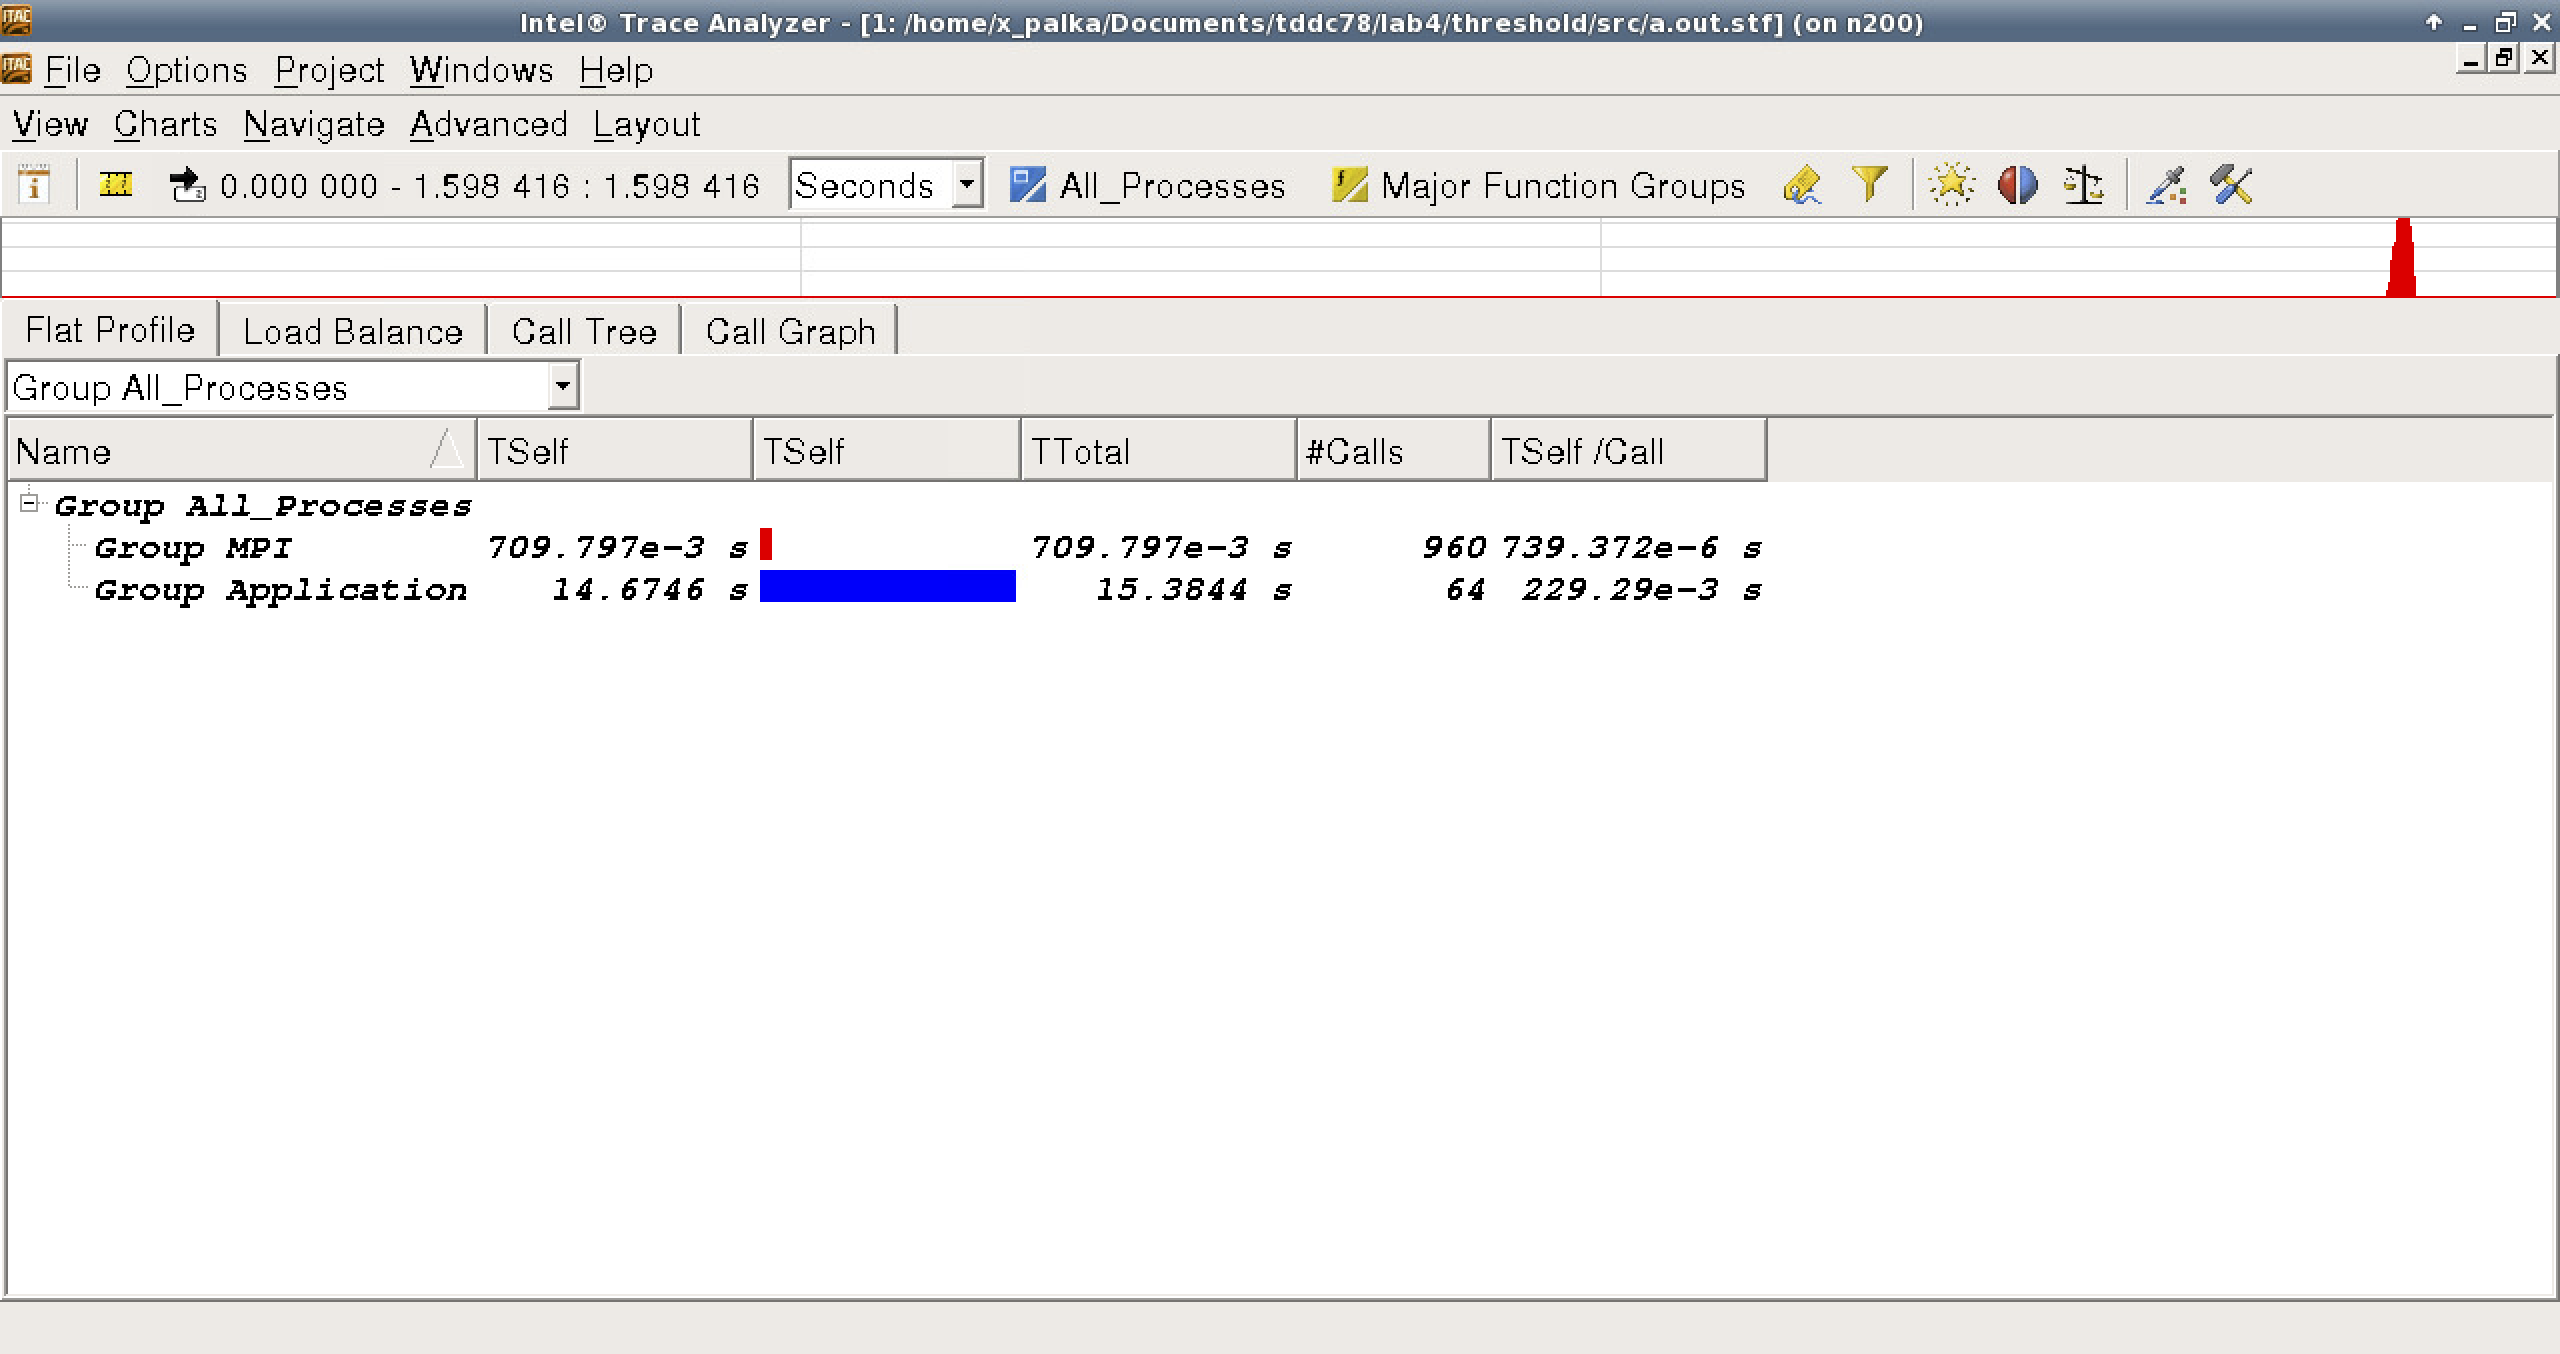
\includegraphics{img/itac.png}}
  \caption{Intel ITAC.}
  \label{fig:itac}
\end{figure}


\end{document}

%% \begin{table}[H]
%%   \centering
%%   \caption{Miss rates}
%%   \begin{tabular}{|*{3}{p{20mm}|}}
%%     \hline
%%     \textbf{Miss rates} & {test1} & {test2} \\ \hline
%%            {cache1} & {0.0091} & {0.1577} \\ \hline
%%            {cache2} & {0.0177} & {0.0235} \\ \hline
%%   \end{tabular}
%%   \label{tab:table1}
%% \end{table}


%% \begin{figure}[H]
%% 	\centering
%% 	\scalebox{0.342}{\includegraphics{img/data-cache.png}}
%% 	\caption{Only data stored in cache.}
%% 	\label{fig:data-cache}
%% \end{figure}

%%thinlinc-und.ida.liu.se
